\documentclass[uplatex, a4paper, 12pt, openany, oneside]{jsbook}

\usepackage[dvipdfmx]{graphicx}
\usepackage[dvipdfmx]{color}
\usepackage[dvipdfmx, bookmarks=true, setpagesize=false]{hyperref}
\usepackage{pxjahyper}

\usepackage{thesis}
\usepackage{here}
\usepackage{url}
\usepackage{subcaption}
\captionsetup[figure]{justification=centering}


\thesis{卒 業 論 文}
\title{
  \centering
    \scalebox{1.0}{視覚と行動のend-to-end学習により経路追従行動を}\\
    \scalebox{1.0}{オンラインで模倣する手法の提案}\\
    \scalebox{0.8}{(オフラインでデータセットを収集して訓練する手法の検証)}
    \vspace{-0.3zh}
    \scalebox{0.7}{A proposal for an online imitation method of path-tracking}
    \scalebox{0.7}{behavior by end-to-end learning of vision and action}
    \scalebox{0.7}{(Validation of a method to collect and train datasets offline)}
    \vspace{-5.0zh}
}
\setlength{\textwidth}{\fullwidth}
\setlength{\evensidemargin}{\oddsidemargin}

\date{\today}
\vspace{-15.0zh}
\teacher{林原 靖男 教授}
\vspace{-15.0zh}
\organization{千葉工業大学 先進工学部 未来ロボティクス学科}
\author{19C1068 髙橋祐樹}
\vspace{-15zh}

\renewcommand{\baselinestretch}{1.2}
\begin{document}

%% Front Matter
\frontmatter{}
%
\chapter{結言}
\label{chap:conclusion}
%
%\input{introduction/preface}
%
%!TEX root = ../thesis.tex

本研究では, 経路追従行動をカメラ画像を入力としたend-to-end学習で模倣する岡田ら\cite{okada-si}と清岡ら\cite{kiyooka-si}の手法を基に, 新たなデータセットの収集方法と収集したデータ量を増やすことで, 経路追従行動を獲得できる手法を提案した. 
%
%
%% Main Matter
\mainmatter{}
%
\chapter{結言}
\label{chap:conclusion}
%
%\input{introduction/preface}
%
%!TEX root = ../thesis.tex

本研究では, 経路追従行動をカメラ画像を入力としたend-to-end学習で模倣する岡田ら\cite{okada-si}と清岡ら\cite{kiyooka-si}の手法を基に, 新たなデータセットの収集方法と収集したデータ量を増やすことで, 経路追従行動を獲得できる手法を提案した. 
%
%
\chapter{要素技術}
\label{chap:technology}
%
%\input{introduction/preface}
%
%!TEX root = ../thesis.tex

\section{ディープラーニング}
ディープラーニングとは, 人間の神経細胞を模したネットワーク構造のことである. 主に, 入力層と出力層, その間に中間層(隠れ層)という構成である. 中間層を多層化することで, 複雑な入力情報を処理し, パターンを認識することや, ルールを読み解くことができる. 近年では, 画像や物体認識, 自然言語処理などで活用されている. \figref{Fig:dl}に構造の一例を示す. 

\vspace{30mm}

\begin{figure}[h]
     \centering
     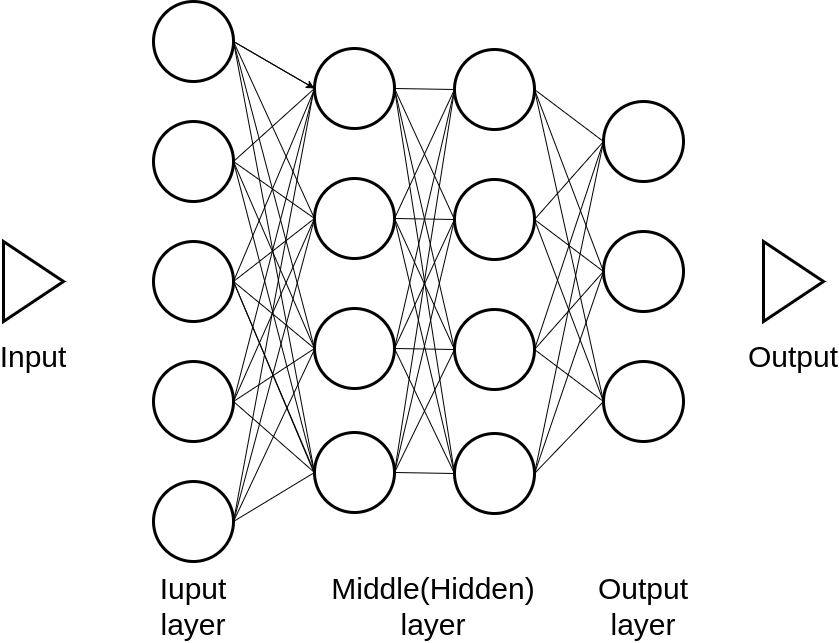
\includegraphics[keepaspectratio, scale=0.3]
     {images/dl.png}
     \caption{Structure of deep learning}
     \label{Fig:dl}
     \end{figure}

\newpage
\section{end-to-end学習}
end-to-end学習とは, 入力から出力までの流れを一括に学習することができる手法である. 例として, 画像中からの文字認識を行う処理を挙げる. 一般的な処理では, \figref{Fig:example}のように画像から文字検出を行い, その後に文字分割, 最終的に文字認識をする. しかし, end-to-end学習では, \figref{Fig:end-to-end}に示すような入力から出力までの流れを一括して学習することができる. 

\vspace{35mm}

\begin{figure}[h]
     \centering
     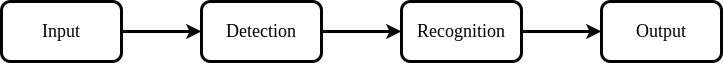
\includegraphics[keepaspectratio, scale=0.5]
     {images/example.png}
     \caption{Structure of general learning}
     \label{Fig:example}
     \end{figure}

\begin{figure}[h]
     \centering
     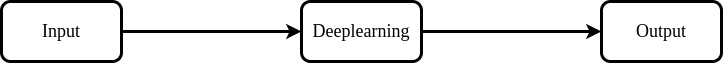
\includegraphics[keepaspectratio, scale=0.5]
     {images/end-to-end.png}
     \caption{Structure of end-to-end learning}
     \label{Fig:end-to-end}
     \end{figure}

\newpage
\section{データセット}
データセットとは, 学習に使用する学習(訓練)データの集合のことである. 例として, \figref{Fig:mnist}に示すような0から9の手書きで書かれた数字の画像セットであるMNISTが挙げられる. 機械学習や画像認識において多く利用されており, 訓練画像6000枚とテスト画像1000枚で構成されている. 

\vspace{5mm}

\begin{figure}[h]
     \centering
     
\includegraphics[keepaspectratio, scale=0.5]
     {images/mnist.png}
     \caption{MNIST dataset(source: \cite{mnist})}
     \label{Fig:mnist}
     \end{figure}

\section{オフライン学習}
オフライン学習とは, あらかじめ用意したデータセットを使用して学習を行うことである. これに対して, 先行研究用で用いたオンライン学習とは, タスクを行いながらデータ収集をし, そのデータを使用して学習することを指す. 

% \section{ミニバッチ学習}
% ミニバッチ学習とは, 訓練データをいくつかのグループ(バッチ)に分けて順番に学習を行うことである. 特徴としては, 勾配更新の頻度が高く, 計算量が少なくて済むといったことが挙げられる. これらの特徴を踏まえて, 先行研究ではオンラインで学習を行うことから, ミニバッチ学習を使用している.
\section{バッチ学習}
バッチ学習とは, 訓練データを一括で処理する学習方法である. 特徴として, 一度に大量のデータを扱うことができるため学習の進行が安定しやすく, 訓練データに異常データが混じっていても受ける影響が小さくて済むなどが挙げられる. また, バッチ学習ではバッチサイズがデータ数となることが多い. 

\section{地図を用いたルールベース制御器によるナビゲーション}
地図を用いたルールベース制御器によるナビゲーションについて説明する. このナビゲーションには, ROSのパッケージであるnavigation\cite{navigation}を使用している. 移動ロボットは, LiDARやホイールオドメトリなどのセンサデータを使用して作成した占有格子地図を用いて目的地まで移動する. そして, 移動ロボットは\figref{Fig:navigation}のように, LiDARやホイールオドメトリなどのセンサデータを入力として, 自己位置推定と経路計画を行い, それらに基づいて自律移動をする. 自己位置推定にはパーティクルフィルタを用いたモンテカルロ自己位置推定(MCL)\cite{mcl1}\cite{mcl2}, 経路計画とモータ指令にはmove\_base\cite{navigation}を使用している.  経路計画では, 動的計画法によって壁や障害物を回避するように経路を生成する. モータ指令は, 生成された経路に従って速度制御を行っている.

% 地図を用いたルールベース制御器によるナビゲーションについて説明する. このナビゲーションには, ROSのパッケージであるnavigation\cite{navigation}を使用している. 移動ロボットは, \figref{Fig:navigation}のようにLiDARのスキャンデータやオドメトリを入力として自己位置推定と経路計画を行い, これらに基づいて自律走行をする. また, 自己位置推定には, amcl(Adaptive Monte Carlo Localization), 経路計画とモータ指令にはmove\_base\cite{navigation}を使用している. 

\begin{figure}[h]
     \centering
     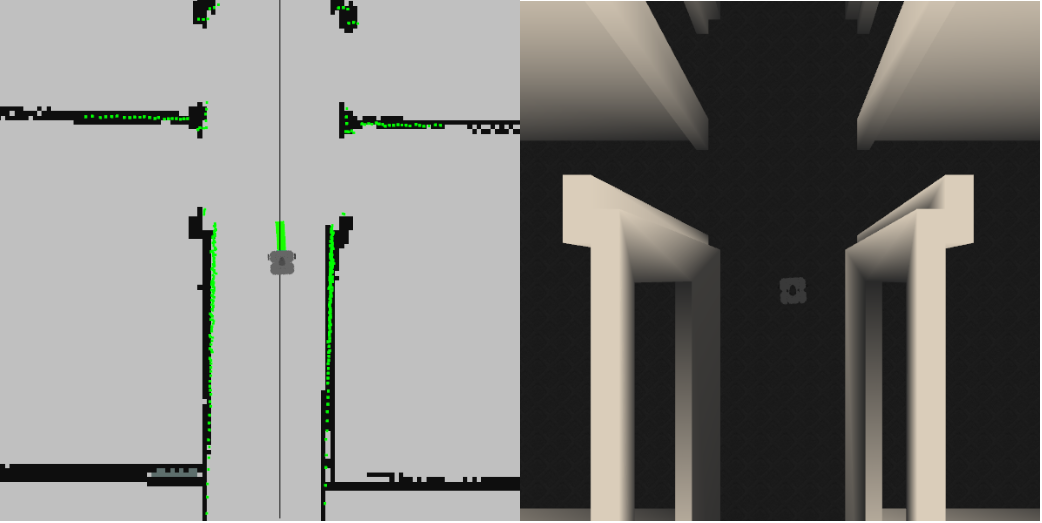
\includegraphics[keepaspectratio, scale=0.3]
     {images/navigation.png}
     \caption{Map based navigation using navigation package}
     \label{Fig:navigation}
     \end{figure}
%
%
\chapter{従来手法}
\label{chap:old-method}
%
%\input{introduction/preface}
%
%!TEX root = ../thesis.tex

\section{従来手法の概要}
従来手法\cite{okada-si2020}では, 地図を用いたルールベース制御器によるナビゲーションの走行を模倣し, 視覚に基づく経路追従行動を獲得した. 従来手法の概要を\figref{Fig:conv-method}に示す. 学習時, 移動ロボットは\figref{Fig:conv-method}(a)に示すようにLiDARとオドメトリを入力とする地図を用いたルールベース制御器によるナビゲーションで走行する. 同時に, 学習器はカメラ画像とナビゲーションの出力であるロボットの目標角速度をend-to-end学習する. 学習後は, \figref{Fig:conv-method}(b)のようにカメラ画像のみを入力とした学習器の出力により走行する. \par また, 1.1章でも述べたように, 目標経路より離れた位置から経路に戻る学習をすることが経路追従をする上で有効である. そのためには, 経路から一度外れる必要がある. しかし, それでは経路から外れる行動も学習してしまう. そこで, 従来手法では, 学習のデータセットに利用する行動と, 学習時にロボットを制御する行動を別々に扱う. これにより, \figref{Fig:old-method3}に示すように経路から離れた位置から経路に戻る行動を学習することができる. 

\newpage
\begin{figure}[h]
  \centering
  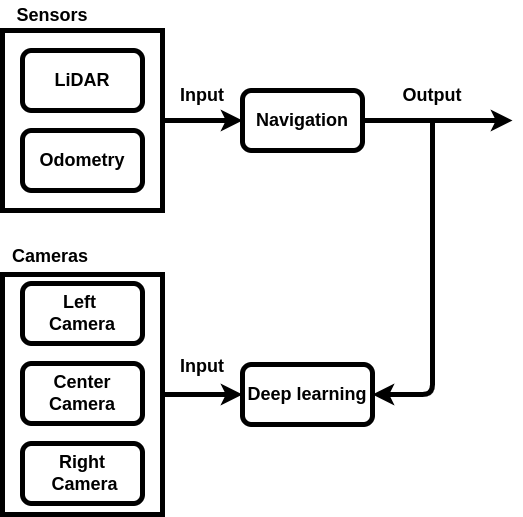
\includegraphics[keepaspectratio, scale=0.36]{images/old-method1.png}
  \caption*{(a)Learning phase}
  \end{figure}

\begin{figure}[h]
  \centering
  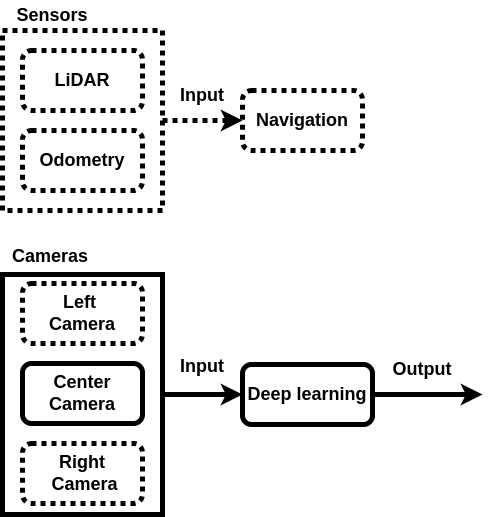
\includegraphics[keepaspectratio, scale=0.36]{images/old-method2.png}
  \caption*{(b)Test phase}
  \caption{Conventional method system}
  \label{Fig:conv-method}
  \end{figure}

% \newpage
% \begin{figure}[h]
%   \begin{minipage}[b]{0.65\linewidth}
%     \centering
%     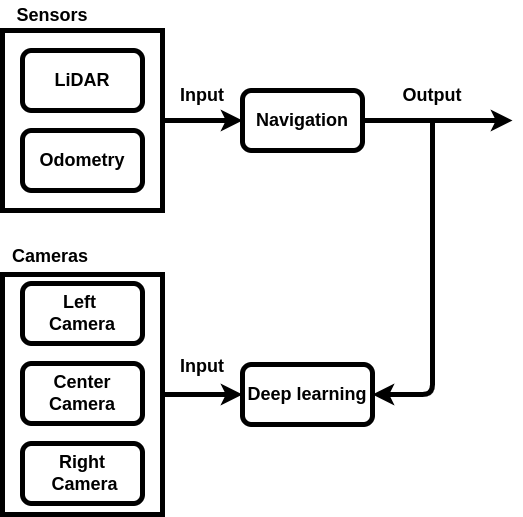
\includegraphics[keepaspectratio, scale=0.4]{images/old-method1.png}
%     \subcaption{Learning phase}
%   \end{minipage}
%   \begin{minipage}[b]{0.45\linewidth}
%     \centering
%     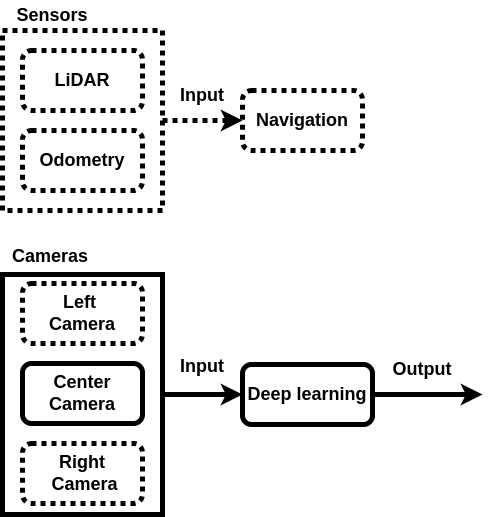
\includegraphics[keepaspectratio, scale=0.4]{images/old-method2.png}
%     \subcaption{Test phase}
%   \end{minipage}
%   \caption{Conventional method system}
%   \label{Fig:conv-method}
% \end{figure}

\newpage
\begin{figure}[h]
  \centering
  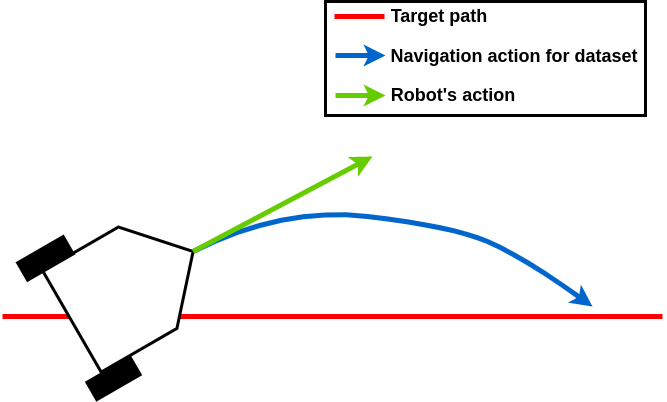
\includegraphics[keepaspectratio, scale=0.4]{images/old-method3.png}
  \caption{The conventional method collects the navigation actions apart from the robot's actions from \cite{okada-si2020}}
  \label{Fig:old-method3}
  \end{figure}

\newpage
\section{従来手法のシステム}
次に, 従来手法のシステムを\figref{Fig:okada-method}に示す. システムでは, LiDAR, オドメトリを入力としたナビゲーションの出力である角速度を学習器とモータ駆動系に与える. ナビゲーションの角速度は, ROSのパッケージであるnavigation\cite{navigation}により計算される. また, 学習器には, カメラ画像を64×48にリサイズした画像を入力し, ナビゲーションの角速度を出力して, 0.2sの周期でend-to-end学習する. 

\vspace{10mm}
\begin{figure}[h]
  \centering
  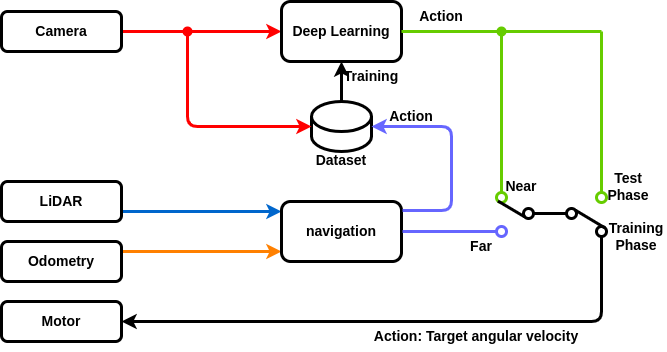
\includegraphics[keepaspectratio, scale=0.45]
  {images/okada-method.png}
  \caption{Systems that imitation learning for map-based navigation from \cite{okada-si2021}}
  \label{Fig:okada-method}
  \end{figure}

  \newpage
\section{ネットワークの構造}
\figref{Fig:cnn}に従来手法で用いたネットワークの構造を示す. 構造は, 入力層1, 畳み込み層3, 全結合層2, 出力層1の計7層から構成されている. また, オンラインで学習が行えるように, ネットワークは畳み込みニューラルネットワーク(CNN)を基にしている. 

\vspace{10mm}
\begin{figure}[h]
  \centering
  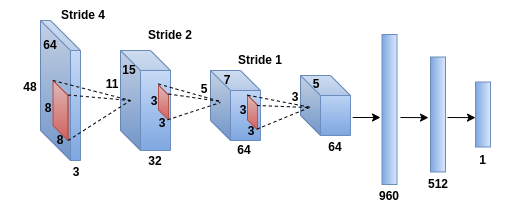
\includegraphics[keepaspectratio, scale=0.6]{images/cnn.png}
  \caption{Structure of network}
  \label{Fig:cnn}
  \end{figure}



%
%
\chapter{提案手法(オフライン手法)}
\label{chap:proposed-method}
%
%\input{introduction/preface}
%
%!TEX root = ../thesis.tex

本章では, 従来研究を基にしたオフラインでデータを収集し訓練する手法を提案する.

\section{手法}
本研究で検証するオフライン手法に関して述べる. オンライン手法と比べて, オフライン手法は画像と目標角速度のデータを事前に収集して, 学習するところが異なる. \figref{Fig:collect-data2}にシミュレータを用いて収集するデータを示す. 目標経路(赤線)から一定距離の位置にロボットを配置して, さらに目標経路の方向を基準として, ヨー方向に一定量回転する. その時の中央のカメラの画像と, 目標角速度を収集してデータセットに加える. ちなみに, 本手法でデータを収集するためには, 非常に多くのロボットの置き直しをしなければならない. これを, 実ロボットに応用する際には, 1台のロボットに複数のカメラを搭載して, 経路から一定距離離れた画像を収集する. そうすることで, 置き直ししなくても経路を走行すればデータを集められる. そのため,実ロボットへの応用も可能であると考える. このように収集したデータセットを用いてオフラインで学習する. なお,リアルタイム性に配慮して, オンライン手法ではバッチサイズ8のミニバッチ学習を行っていたが, オフライン学習ではリアルタイム性は必要ないため, バッチ学習を行う. 

% \vspace{10mm}
\newpage
  \begin{figure}[h]
  \centering
  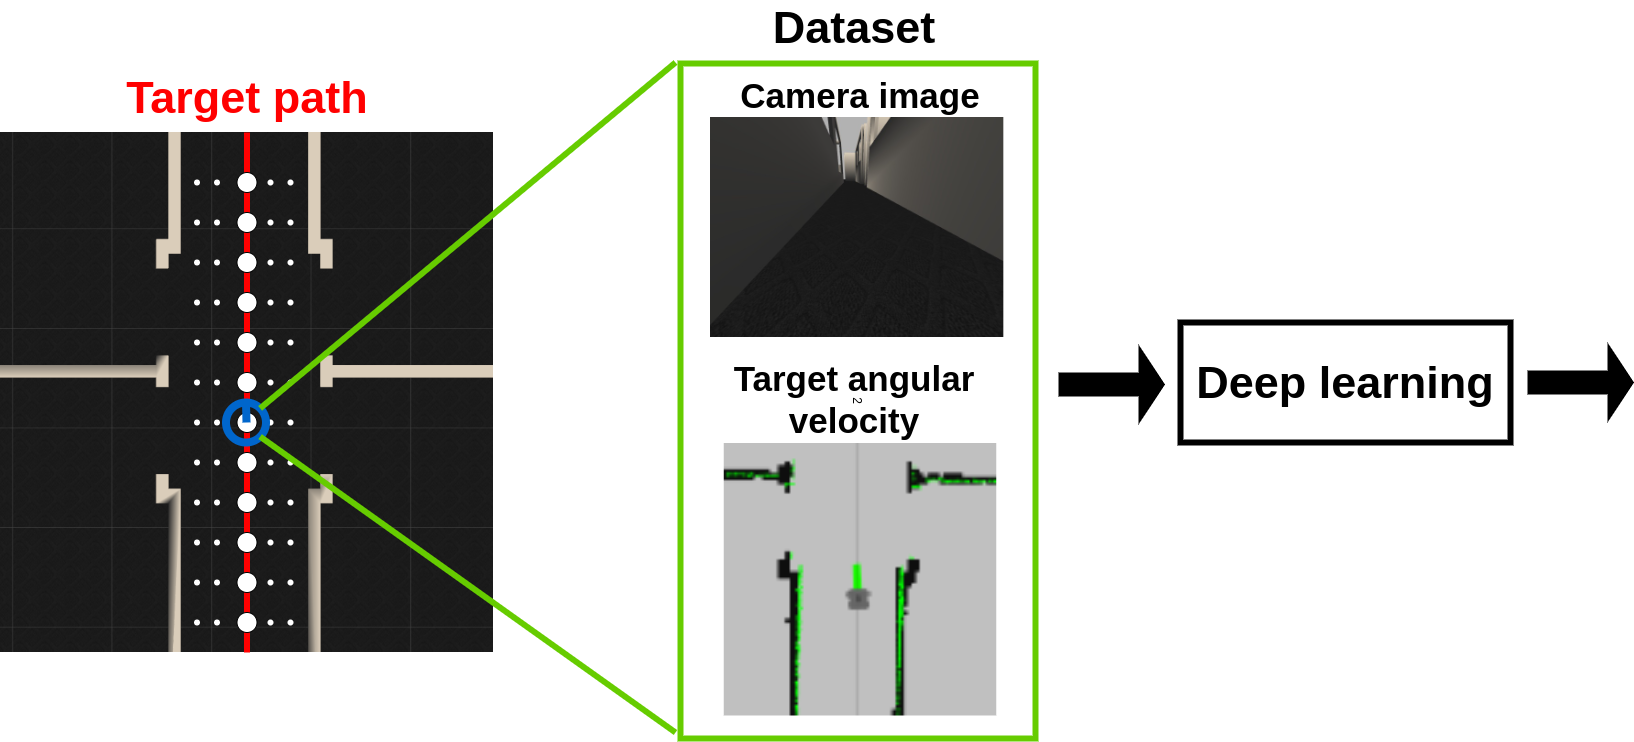
\includegraphics[keepaspectratio, scale=0.2]{images/collect-data2.png}
  \caption{Data collected by the simulator in the learning phase}
  \label{Fig:collect-data2}
  \end{figure}


%
%
\chapter{提案手法(オフライン手法)}
\label{chap:experiment}
%
%\input{introduction/preface}
%
%!TEX root = ../thesis.tex

\section{実験概要}
本章では, 提案手法の有効性を検証する. そのためにシミュレータを用いた実験を行う. 実験はロボットの位置と向きを組み合わせた全8パターンで検証する. それぞれの組み合わせでデータを収集して学習し, 成功率を比較する. 

\section{実験装置}
実験環境は, \figref{Fig:gazebo}に示すGazebo\cite{gazebo}のWillow Garage\cite{willow}を使用して, \figref{Fig:willow-garage}に示す赤線を目標経路として実験する. ロボットモデルには\figref{Fig:turtlebot3}に示すようなカメラを1つ搭載したTurtlebot3\cite{turtlebot3}を用いた. 

\begin{figure}[h]
  \centering
  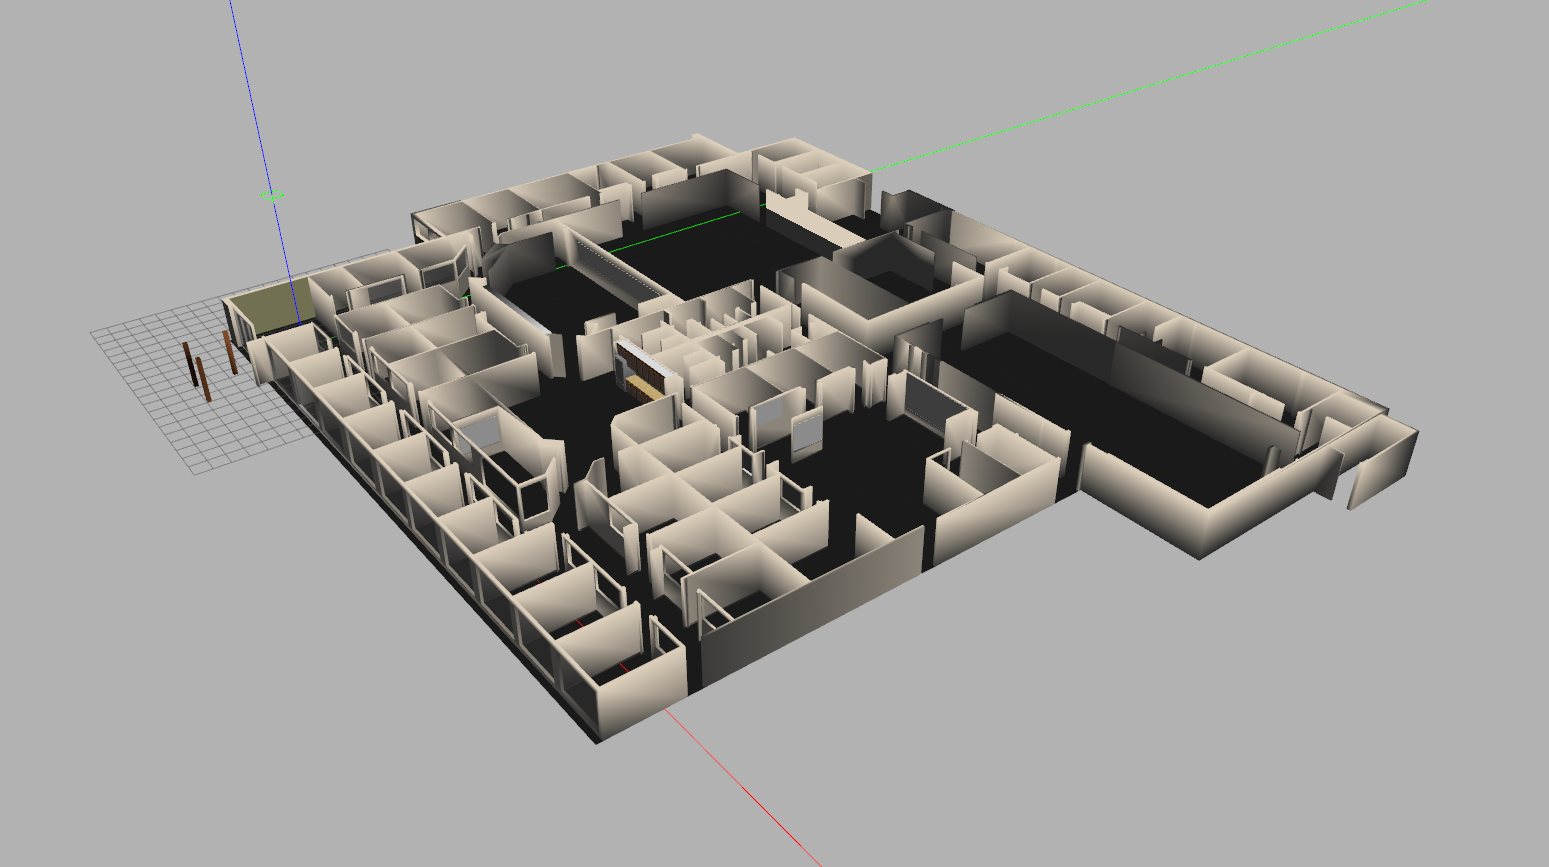
\includegraphics[keepaspectratio, scale=0.15]{images/gazebo.png}
  \caption{Experimental environment in simulator}
  \label{Fig:gazebo}
  \end{figure}

\newpage
\vspace{20mm}
\begin{figure}[h]
  \centering
  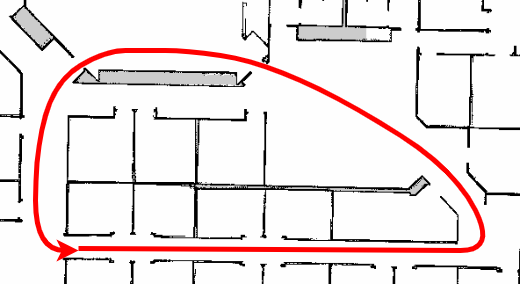
\includegraphics[keepaspectratio, scale=0.5]{images/willow-path.png}
  \caption{Course to collect data}
  \label{Fig:willow-garage}
  \end{figure}

\begin{figure}[h]
  \centering
  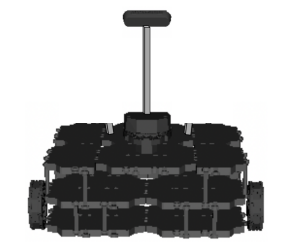
\includegraphics[keepaspectratio, scale=0.55]{images/1cam_turtlebot3.png}
  \caption{Turtlebot3 waffle with a camera}
  \label{Fig:turtlebot3}
  \end{figure}

\newpage
\section{実験方法}
\begin{description}
  \item[1)データ収集]\mbox{}\\ \hspace*{3mm}データの収集方法について述べる. \figref{Fig:old-method}にデータの収集方法を示す. 図のようにロボットを目標経路上と目標経路から±0.1[m], ±0.2[m], ±0.3[m]の位置に配置する. 位置に関する実験条件は, 以下の4種類となる. 
  \par (a)目標経路上のみ
  \par (b)目標経路上と目標経路から±0.1[m]の位置
  \par (c)目標経路上と目標経路から±0.2[m]の位置
  \par (d)目標経路上と目標経路から±0.3[m]の位置
  \vskip\baselineskip
  \par \hspace*{3mm}また, 各位置において, 目標経路の向きを基準として, ロボットをヨー方向に0[deg]と±5[deg]回転させる. 角度に関する実験条件は, 以下の2種類となる. 
  \par (e)目標経路の向きと±5[deg]回転させた向き
  \par (f)目標経路の向きのみ
\end{description}

\begin{figure}[h]
  \centering
  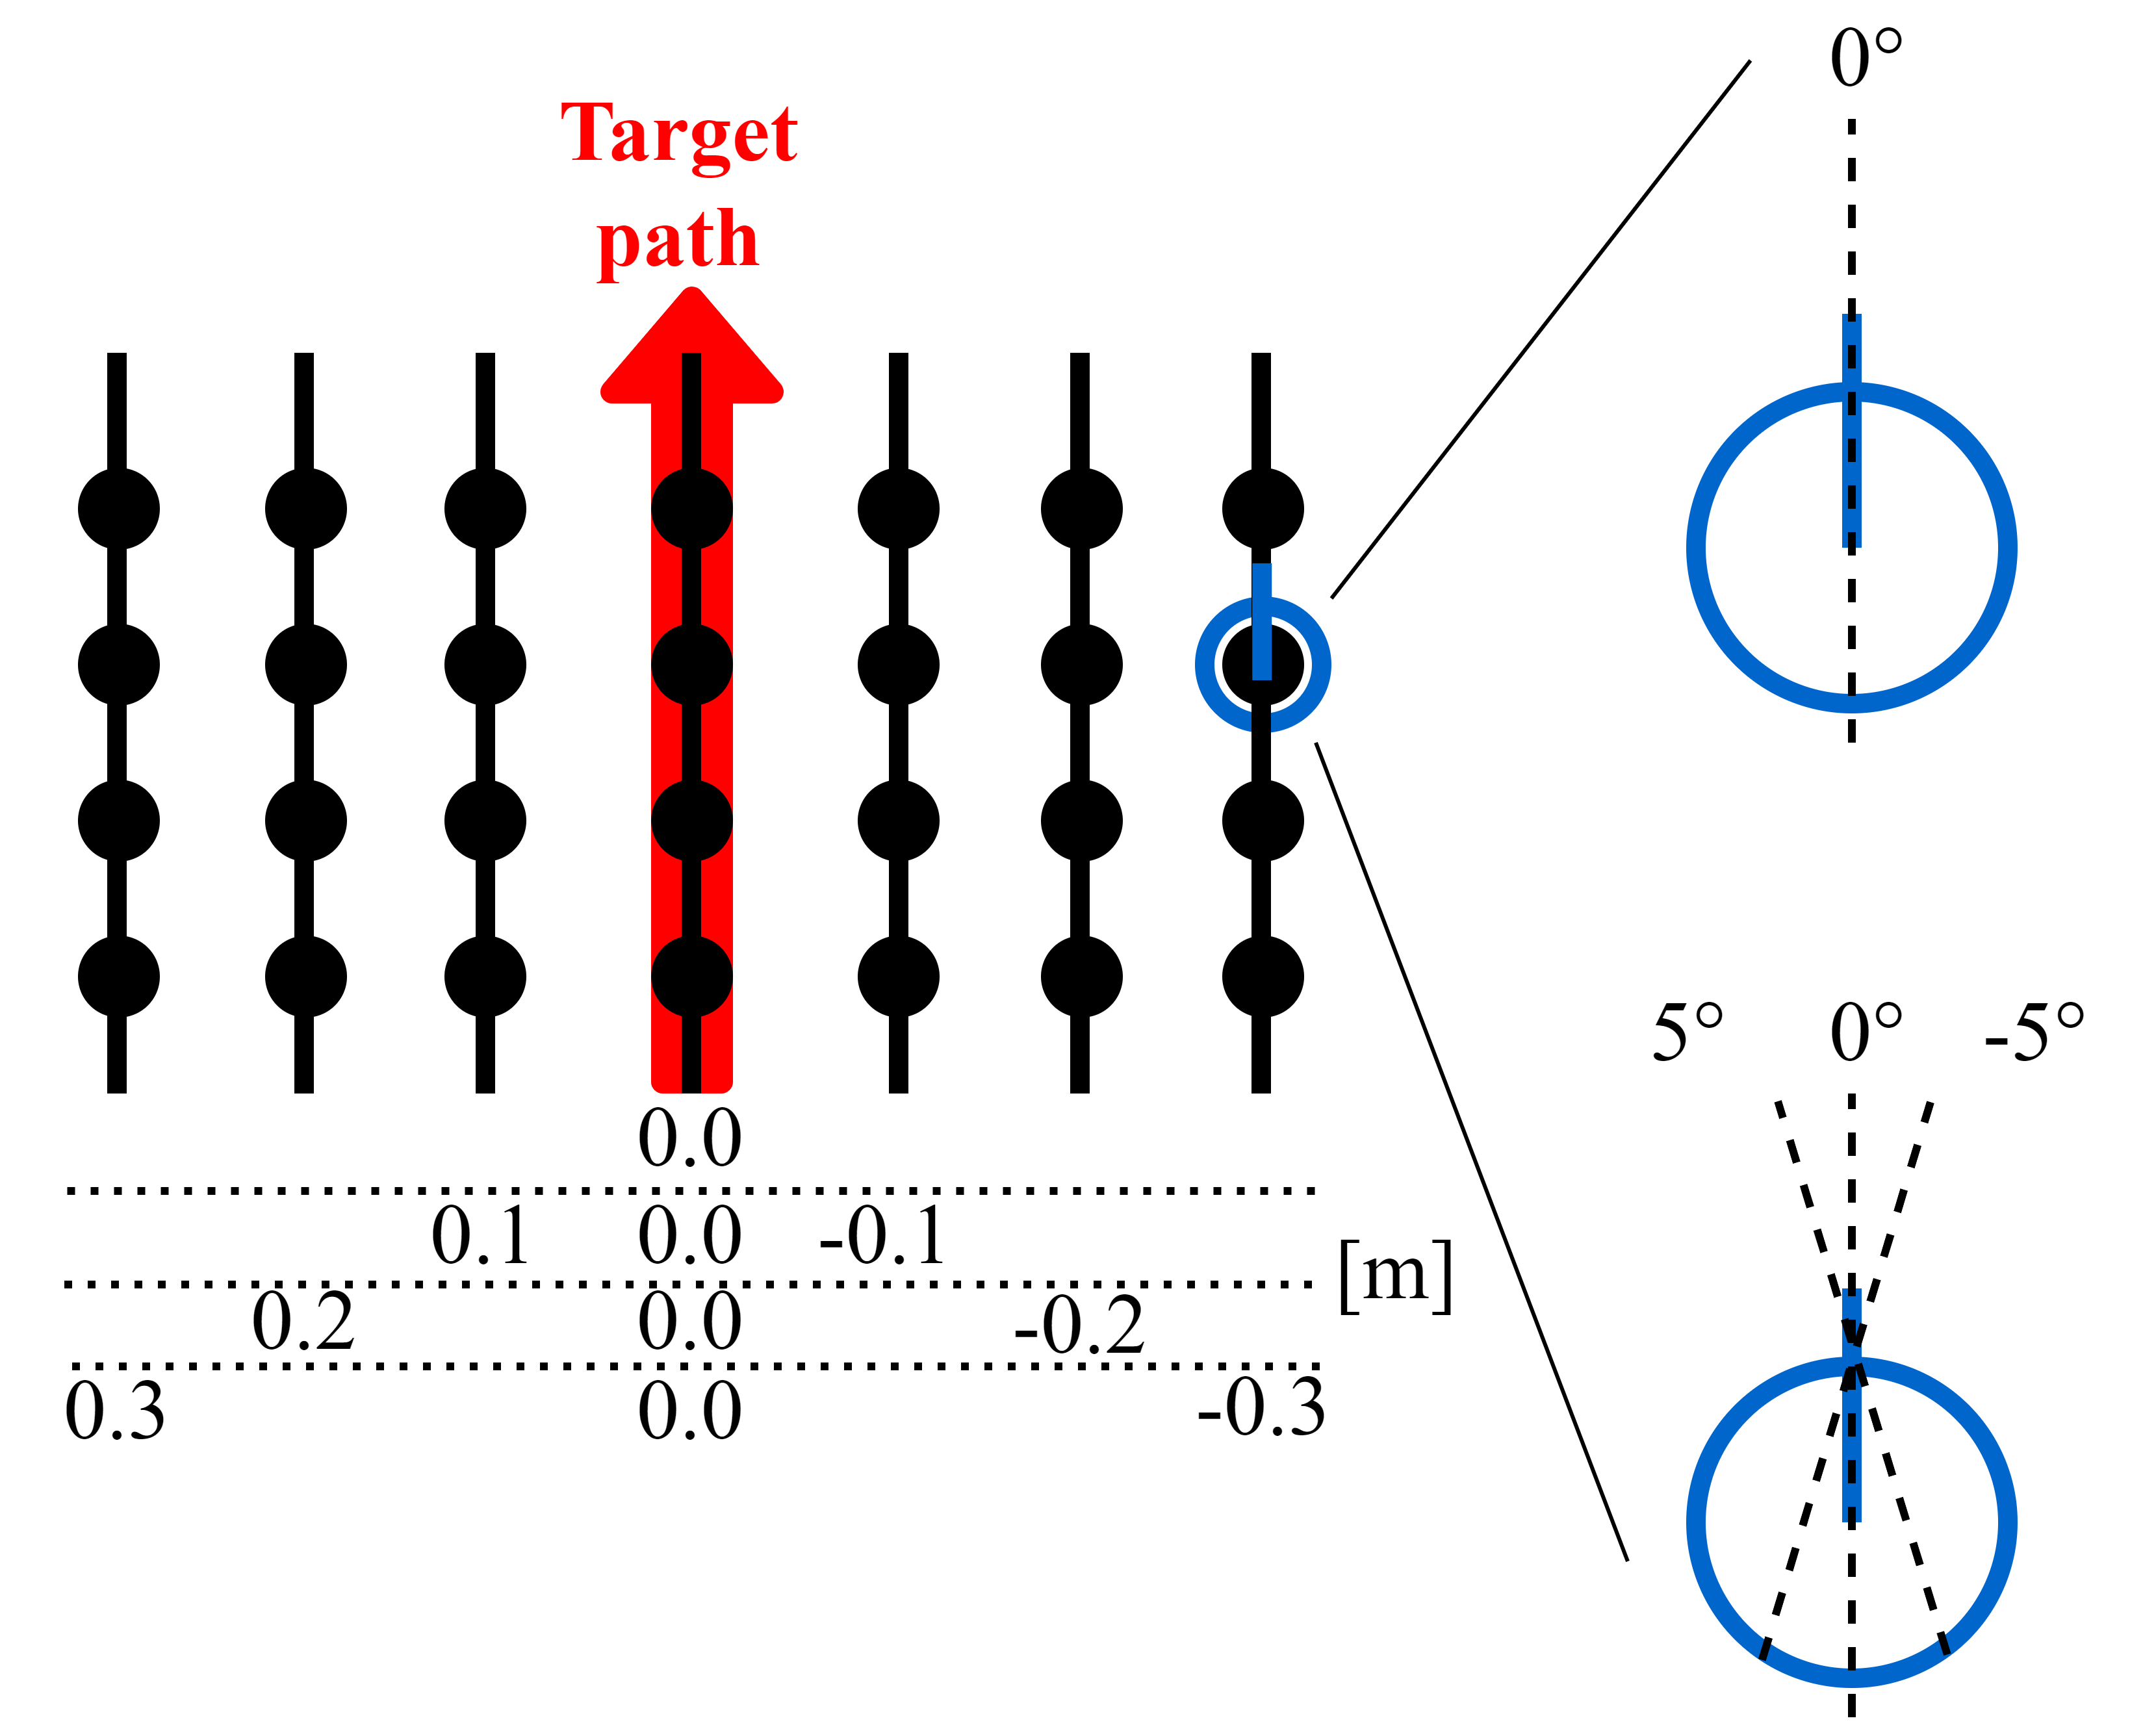
\includegraphics[keepaspectratio, scale=0.6]{images/collect2.png}
  \caption{Location and orientation of the robot in the experiments}
  \label{Fig:old-method}
  \end{figure}

\begin{description}
  \item[2)訓練]\mbox{}\\ \hspace*{3mm}収集したデータを用いて, バッチ学習を4000step行う. なお, オンライン手法では同様の条件で8000step行っていた. オフライン手法では, 後に述べるように4000stepでlossがほぼ収束するため, 4000stepを採用した.
\end{description}

\begin{description}
  \item[3)テスト]\mbox{}\\ \hspace*{3mm}学習したモデルを用いてロボットを走行させ, \figref{Fig:willow-garage}に示した目標経路を追従できるかを検証する. ロボットの並進速度0.2m/sとし, 経路を1周できた場合を成功とし, 壁に激突した場合を失敗とした. 上記の2)学習と3)テストを30回行い, 経路追従の成功回数を求めた. 
\end{description}

\section{実験結果と考察}
実験結果を表\ref{tb:exp1}に示す. 列は位置の4条件(a)~(d)を並べたものであり, 行は方向の2条件(e), (f)を並べたものである. 分母の30は実験回数を示しており, 分子の数は成功回数を示している. 結果的に, 目標経路上及び±0.2[m]の位置, 0[deg]及び±5[deg]の向きに, ロボットを配置する条件で100%(30回中30回)成功している. これは, オンライン手法において最も高い成功率100%\cite{okada-si2021}と同じである. オンライン手法が40分程度必要なのに対して, オフライン手法での学習時間は4分程度であったことから, 学習に要する時間を1/10に短縮できることを確認できた. ただし, オフライン手法での学習時間4分には, 実験方法で述べたデータ収集は含まれていない. 

\begin{table}[h]
  \centering
  \caption{Number of successes in the batch learning}
  \begin{tabular}{|p{2cm}|p{2cm}|p{2cm}|p{2cm}|p{2cm}|} \hline
     & 0[m] & 0, ±0.1[m] & 0, ±0.2[m] & 0, ±0.3[m] \\ \hline
    0, ±5[deg] & 1/30 & 28/30 & \bf30/30 & 27/30 \\ \hline
    0[deg] & 0/30 & 14/30 & 23/30 & 20/30 \\ \hline
  \end{tabular}
  \label{tb:exp1}
\end{table}

ここで, \figref{Fig:loss_00_02_4000}に, この実験条件で学習したときのlossグラフを示す. 図から4000stepでlossがほぼ収束している様子が見られる. 

\newpage
\begin{figure}[h]
  \centering
  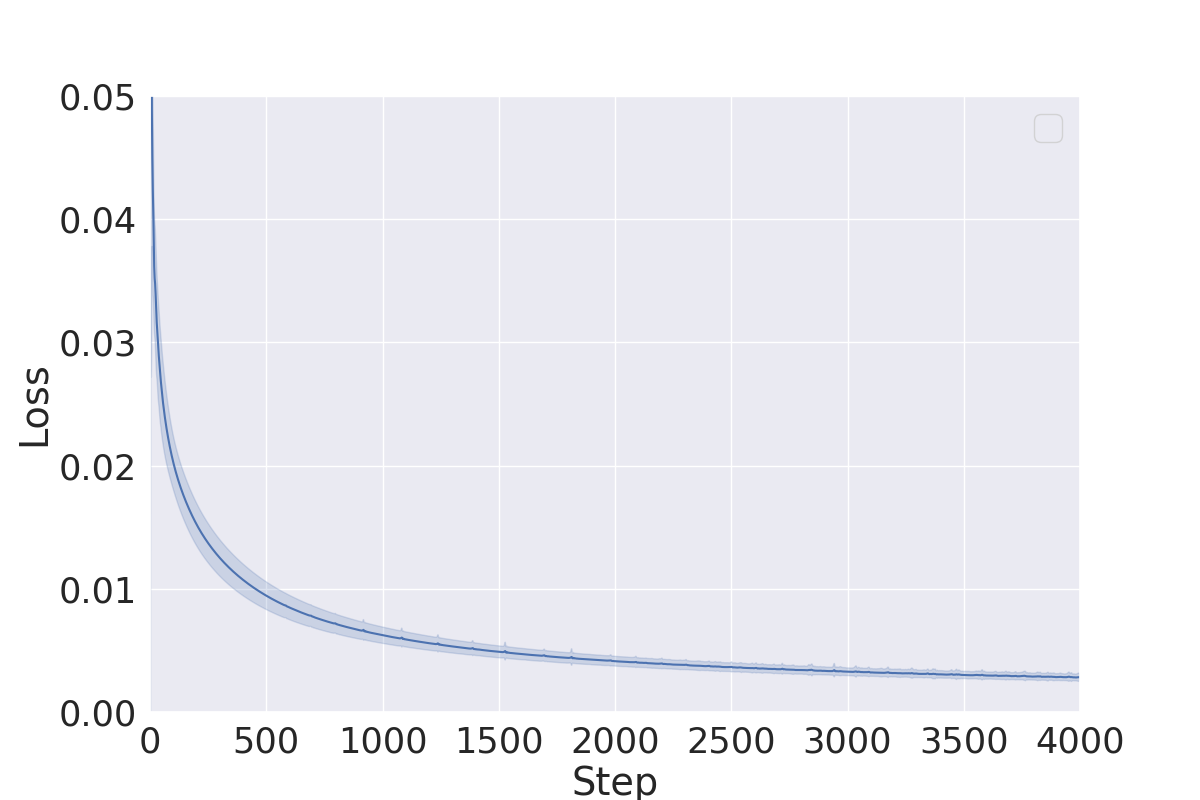
\includegraphics[keepaspectratio, scale=0.35]{images/loss_00_02_4000.png}
  \caption{Loss value in the experiment}
  \label{Fig:loss_00_02_4000}
  \end{figure}

また, \ref{tb:exp1}の他の結果を見ると, 30回成功した実験条件(位置0[m], ±0.2[m], 向き0[m], ±5[deg])から離れるほど成功率が低くなっている. 特にカメラの方向が0[deg]のみの場合は顕著に成功率
が低くなっている. また, 目標経路上の画像しか使用しない条件(位置0[m])では, ほとんど成功していない. それ以外の実験条件でも, カメラ間の距離により成功率が変化する様子が見られているが, この原因の究明は今後の課題としたい. 

\section{まとめ}
本章では, 事前に収集した画像と行動を用いて, end-to-end学習により経路追従行動をオフラインで模倣学習する手法に関して検討した. シミュレータを用いた実験により, 以下のことを確認した. 

\begin{itemize}
  \item 目標経路上及び±0.2[m]の位置, 0[deg]及び±5[deg]の向きの視覚情報があれば経路追従できることを確認
  \item オンライン手法で問題となっていた学習に要する時間を1/10に短縮できることを確認
\end{itemize}
%
%
\chapter{結言}
\label{chap:conclusion}
%
%\input{introduction/preface}
%
%!TEX root = ../thesis.tex

本研究では, 経路追従行動をカメラ画像を入力としたend-to-end学習で模倣する岡田ら\cite{okada-si}と清岡ら\cite{kiyooka-si}の手法を基に, 新たなデータセットの収集方法と収集したデータ量を増やすことで, 経路追従行動を獲得できる手法を提案した. 
%
%% Back Matter
\backmatter{}
%
%!TEX root = ../thesis.tex
%\bibliographystyle{plain}
\bibliographystyle{junsrt}
%\bibliography{report}
\nocite{*}
% \bibliography{main_bibliography}
%!TEX root = ../thesis.tex
% \chapter*{参考文献}
\addcontentsline{toc}{chapter}{参考文献}

\begin{thebibliography}{99}

  \bibitem{okada-si2020}
  岡田 眞也, 清岡 優祐, 上田 隆一, 林原 靖男: ``視覚と行動のend-to-end学習により経路追従行動をオンラインで模倣する手法の提案'', \textit{計測自動制御学会 SI 部門講演会 SICE-SI2020 予稿集}, pp.1147-1152, 2020.

  \bibitem{okada-si2021}
  岡田 眞也, 清岡 優祐, 春山 健太, 上田 隆一, 林原 靖男: ``視覚と行動のend-to-end学習により経路追従行動をオンラインで模倣する手法の提案 -経路追従行動の修正のためにデータセットを動的に追加する手法の検討'', \textit{計測自動制御学会 SI 部門講演会 SICE-SI2021 予稿集}, pp.1066-1070, 2021.

  \bibitem{bojaski}
  Mariusz Bojarski et al., ``End to End Learning for Self-Driving Cars.'', arXiv: 1604.07316(2016). 

  \bibitem{Jing}
  Jing Bi, Tianyou Xiao, Qiuyue Sun, Chenliang Xu., ``Navigation by Imitation in a Pedestrian-Rich Environment,'' arXiv preprint arXiv:1811.00560, 2018.

  \bibitem{navigation}
  ros-planning, navigation
  \url{https://github.com/ros-planning/navigation}
  (最終閲覧日: \today)

  \bibitem{mcl1}
  F. Dellaert, Fox D., Burgard W., and S Thrun. “Monte carlo localization for mobile robots“. Proceedings 1999 IEEE international conference on robotics and automation (Cat. No. 99CH36288C), Vol. 2, pp. 1322–1328, 1999.

  \bibitem{mcl2}
  D. Fox, W. Burgard, F. Dellaert, and S. Thrun. “ Monte carlo localization: Efficient position estimation for mobile robots“. AAAI/IAAI, Vol. 2-2, pp. 343–349, 1999.

  \bibitem{mnist}
  The MNIST database of handwritten digits
  \url{http://yann.lecun.com/exdb/mnist/}
  (最終閲覧日: \today)

  \bibitem{offline}
  髙橋 祐樹, 白須 和暉, 藤原 柾, 上田 隆一, 林原 靖男: ``視覚と行動のend-to-end学習による経路追従行動の模倣 -データセットを収集してオフラインで訓練する手法の検討-'', 日本機械学会ロボティクス・メカトロニクス講演会2023講演論文集, 2P1-G07, 2023.

  \bibitem{gazebo}
  gazebo.
  \url{http://gazebosim.org/.}
  (最終閲覧日: \today)

  \bibitem{willow}
  Koenig and Nathan and Andrew Howard., ``Design and use paradigms for gazebo, an open-source multi-robot simulator.'' 2004 IEEE/RSJ International Conference on Intelligent Robots and Systems (IROS)(IEEE Cat. No. 04CH37566). Vol. 3. IEEE, pp.2149-2154(2004).
  (最終閲覧日: \today)

  \bibitem{turtlebot3}
  Turtlebot3 — robotis emanual.robotis.
  \url{https://emanual.robotis.com/docs/}
  (最終閲覧日: \today)

\end{thebibliography}
% \input{main_bibliography}
%
%!TEX root = ../thesis.tex
\chapter*{付録}
\addcontentsline{toc}{chapter}{付録}
成功や失敗した際のロボットの走行の軌跡を掲載(一例)

%
%!TEX root = ../thesis.tex
\chapter*{謝辞}
\addcontentsline{toc}{chapter}{謝辞}

本研究を進めるにあたり,1年に渡り, 熱心にご指導を頂いた林原靖男教授に深く感謝いたします.また, 日頃から研究へのアドバイス, 指導, サポートしてくださった清岡優祐様, 春山健太様, 藤原柾様, 白須和暉様, 並びにロボット設計制御研究室の皆様には, 心から深く感謝を申し上げます. 
%


%

\end{document}
